Tässä luvussa esitetään perusteet ja tarvittavat tiedot ohjelmistojen testauksesta ja testiautomaatiosta, jotka liittyvät työn laajempaan teoreettiseen kehykseen.
Ensin esitetään testiautomaation tarkoitus, jonka jälkeen käydään yksityiskohtaisesti läpi ohjelmistotestauksen tasot ja pohditaan niiden merkitystä testiautomaatiossa.
Lopuksi vielä esitetään tarvittavia jatkuvan integroinnin ja testausvetoisen kehityksen perusteita sekä pyritään luomaan ymmärrystä siitä miten ne liittyvät niitä laajempaan testiautomaation käsitteeseen.
Testiautomaation perusteiden ymmärtämistä tarvitaan varsinkin työn myöhemmässä vaiheessa, jossa esitetään varsinainen testitapauksien priorisointi painotetun verkon avulla.

\section{Testiautomaation tarkoitus} \label{ch:07_testiautomaation_tarkoitus}

Testiautomaation tarkoitus on pohjimmiltaan mahdollistaa ohjelmistotuotteen jatkuva ja vaivaton laadunvarmistus, nyt ja tulevaisuudessa.
Testiautomaation vastakohtana voidaan ajatella manuaalista testausta, joka vaatii ihmisen interaktiota testauksen suorittamiseen.
Testiautomaatiossa käytetään erityisiä ohjelmistotyökaluja ennalta määritettyjen testitapauksien suorittamiseen, ihmisen tekemän manuaalisen testauksen sijaan.
Ohjelmistojen testaamisella itsessään pyritään löytämään ohjelmistotuotteesta virheitä, anomalioita ja varmistamaan, että se toimii asetettujen vaatimusten mukaisesti.
Testauksen automatisoiminen vapauttaa aikaa, kustannuksia ja henkilöresursseja manuaalisesta testaamisesta muihin tuotantotehtäviin sekä parantaa toistuvien testien luotettavuutta poistamalla manuaalisessa testauksessa tapahtuvat inhimillisen virheet.
Testiautomaatiolla, joka kytketään osaksi ohjelmistotuotantoprosessia, voidaan myös löytää ohjelmistokehityksen aikana ohjelmistokoodiin lipsuvia virheitä ja näin ollen saavuttaa mahdollisuus korjata niitä ennen kuin ohjelmisto julkaistaan loppukäyttäjille.

Laadunvarmistuksen osalta ohjelmistokehityksessä on usein käytetty niin sanottuja laadullisia ominaisuuksia, joiden kattamisella voidaan validoida laatua.
Laadullisia ominaisuuksia ovat ISO 9126-standardin mukaan: toiminnallisuus, luotettavuus, käytettävyys, tehokkuus, ylläpidettävyys ja siirrettävyys \parencite{iso_9126-1_2001}.
Näistä laadullisista ominaisuuksista testiautomaatiolla pystytään kattamaan erityisesti toiminnallisia, luetettavuudellisia ja tehokkuudellisia ominaisuuksia.
Käytettävyyden, ylläpidettävyyden ja siirrettävyyden validointi puolestaan on vaikeaa testiautomaation avulla, sillä ne ovat varsin subjektiivisia.
Tässä diplomityössä testiautomaation yhteydessä keskitytään erityisesti toiminnallisiin laatuominaisuuksiin ja niiden testaamiseen.

\section{Testauksen tasot} \label{ch:07_testauksen_tasot}

Testauksen tasoja on useita ja usein ohjelmistojen kattavaan testaamiseen on suositeltavaa käyttää ohjelmistotuotantoprosessissa eri tasojen yhdistelmää.
Ohjelmistojen testaus usein jaotellaan kolmeen erilaiseen menetelmään, jotka myös vaikuttavat eri testauksen tasojen käyttökelpoisuuteen.
Erilaisia menetelmiä ovat mustalaatikkotestaus, harmaalaatikkotestaus ja valkolaatikkotestaus, jotka eroavat toisistaan yleisesti ottaen siinä, otetaanko tieto ohjelmistotuotteen sisäisestä toteutuksesta mukaan testaamiseen.
Testauksen tasot esitetään kirjallisuudessa usein hieman eri muodoissa, mutta yleisesti ne jaetaan neljään eri tasoon, jotka voidaan kuvata pyramidin tasoavaruuteen projisoituna muotona.

\begin{figure}[H]
  \centering
  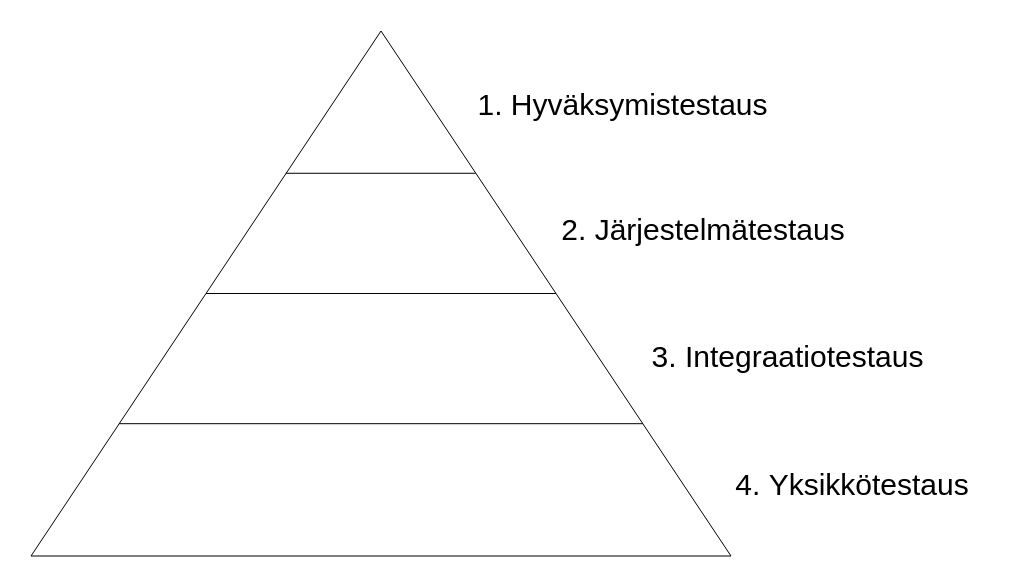
\includegraphics[width=0.8\textwidth]{assets/testing-levels-pyramid.png}
  \caption{Testauksen tasot pyramidin muodossa}
  \label{fig:testing_levels_pyramid}
\end{figure}

Pyramidimuodossa esitetyistä testauksen tasoista kaikkiin on mahdollista soveltaa testiautomaatiota.
Pyramidimuodossa alimpana kuvataan aina yksikkötestaus, joka on tasoista atomisin ja myös luo vahvan pohjan kokonaisvaltaiselle testaamiselle.
Noustessa pyramidissa ylöspäin testattavana olevan kohteen laajuus ja kompleksisuus kasvaa.
Ylimpänä pyramidissa on hyväksymistestaus, joka on tarkoituksellista toteuttaa vaatimusmäärittelyn täyttävää valmista järjestelmää vastaan.
Hyväksymistestaus on tämän diplomityön keskiössä ja siihen liittyvää teoriaa esitetään vielä laajemmin hyväksymistestaus-luvussa \ref{ch:08_hyvaksymistestaus}.
Seuraavissa kappaleissa esitetään vielä yksityiskohtaisemmin jokainen pyramidissa \ref{fig:testing_levels_pyramid} esitetty testauksen taso.

  \subsection{Yksikkötestaus} \label{ch:07_yksikkotestaus}

  Yksikkötestauksen ajatuksena on testata ohjelmistotuotteen lähdekoodista löytyviä yksiköitä, kuten luokkia, funktioita tai moduleita.
  Yksikkötestaus toteutetaan ohjelmiston toteuttavia pienimpiä yksikköjä vastaan ja sen avulla pyritään validoimaan, että jokainen yksikkö toimii siten kuin ne on ohjelmistokehityksessä suunniteltu toimimaan.
  Yksikkötestaus eroaa muista testauksen tasoista siinä, että sen voi suorittaa ainoastaan ohjelmistokehittäjät tai muut ohjelmiston lähdekoodiin perehtyneet henkilöt.
  Yksikkötestauksella pyritään varmistamaan, että ohjelmiston pienimmät yksiköt toimivat tarkoituksenmukaisella tavalla.

  Yksikkötestausta hyödynnetään usein myös ketterien menetelmien aihepiirissä, jossa ohjelmistotuotanto voidaan toteuttaa muun muassa niin sanotulla testausvetoisella kehityksellä \ref{ch:07_testausvetoinen_kehitys}.
  Testausvetoisessa kehityksessä ohjelmistokehittäjät laativat ensisijaisesti yksiköiden yksikkötestit ennen niiden toteuttamisen aloittamista.
  Ohjelmistotestauksen tasojen pyramidissa ja hyvin toteutetussa ohjelmistotestauksen kaikki tasot kattavassa testauksessa tämä testauksen taso on kaikista laajin.
  Monitasoisessa testauksessa yksikkötestaus luo tärkeän pohjan testaamiselle kokonaisuutena ja antaa tietoa ohjelmiston pienimpien yksiköiden toimivuudesta.
  Yksikkötestaus on myös paljon käytetty ja tärkeä osa testiautomaatiossa, sillä se varmistaa sovelluksen yksiköiden suunniteltua toimintaa.

  \subsection{Integraatiotestaus} \label{ch:07_integraatiotestaus}

  Integraatiotestauksen ajatuksena on testata ohjelmistotuotteen toteuttavien eri komponenttien yhteentoimivuutta niiden rajapintojen osalta.
  Integraatiotestaus toteutetaan ohjelmiston suunnitelmaa ja mallia vastaan.
  Integraatiotestauksen onnistuminen luo perustan ohjelmiston toimimiseen ja koostamiseen kokonaisena, eri komponenteista koostuvana järjestelmänä.

  Integraatiotestauksen yhteydessä puhutaan usein myös niin sanotusta savutestauksesta, jonka tarkoituksena on koostaa päivittäinen koontiversio ohjelmistosta ja testata sen kriittisten komponenttien yhteentoimivuus.
  Integraatiotestaus on myös tärkeä osa testiautomaatiosta, sillä sen avulla voidaan varmistaa sovelluksen yksiköiden, kuten esimerkiksi luokkien, komponettien tai modulien yhteentoimivuus.

  \subsection{Järjestelmätestaus} \label{ch:07_jarjestelmatestaus}

  Järjestelmätestauksen ajatuksena on testata kokonaista ja toimivaa järjestelmää, yhtenä suurena yksikkönä.
  Järjestelmätestaus toteutetaan usein eräänlaisena tulikokeena, erityisesti ohjelmiston vaatimuksia vastaan.
  % TODO lisää tekstiä..

  Järjestelmätestaukseen liittyy laajasti erilaisia testattavia laadullisia ominaisuuksia, kuten toiminnallisuus, luotettavuus, käytettävyys, tehokkuus, ylläpidettävyys ja siirrettävyys.
  Aiemmin testiautomaation tarkoitus kappaleessa \ref{ch:07_testiautomaation_tarkoitus} esitettiin, näistä laadullisista ominaisuuksista kaikki eivät sovellu hyvin testiautomaation avulla testattaviksi.
  Tästä syystä järjestelmätestauksella voidaan automatisoidusti testata lähinnä ohjelmiston toiminnallisuutta, luotettavuutta ja tehokkuutta.
  Sen myötä testauksen tasona se on testiautomaation kannalta hyvin samanlainen kuin sitä spesifimpi hyväksymistestaus.
  Joissakin yhteyksissä järjestelmätestaus ja hyväksymistestaus esitetään jopa yhteisenä testauksen tasona, koska testiautomaation kannalta ne muistuttavat kovasti toisiaan.
  Järjestelmätestaus, osittain hyväksymistestauksen kanssa on erittäin merkittävä osa testiautomaatiosta, sillä sen avulla voidaan varmistaa kokonaisen järjestelmän toiminnallisuus.

  \subsection{Hyväksymistestaus} \label{ch:07_hyvaksymistestaus}

  Hyväksymistestauksen ajatuksena on varmistaa toteutettavan ohjelmiston vaatimusten toimivuus erityisesti käytännön tilanteissa.
  Hyväksymistestaus toteutaan ohjelmiston toimintoja kuvaavaa vaatimusmäärittelyä vastaan.
  Hyväksymistestaus on tarkoituksenmukaista laatia sellaiseen muotoon joka testaa lopullisten käyttäjien toimintaa vastaavia käyttötilanteita.
  Samassa asiayhteydessä puhutaan usein myös niin sanotusta päästä päähän testauksesta (englanniksi: e2e, end-to-end).
  Testiautomaatio on erittäin hyödyllinen hyväksymistestausen osalla, koska sillä voidaan automatisoida ohjelmiston validointi ja hyväksyminen sekä estää puutteellisesti toimivan ohjelmiston julkaiseminen.
  % TODO lisää tekstiä..

  Hyväksymistestaus, osittain järjestelmätestauksen kanssa on äärimmäisen merkittävä osa testiautomaatiosta, sillä sen avulla voidaan varmistaa kokonaisen järjestelmän toiminnallisuus ja verifioida, että se vastaa vaatimusmäärittelyä.
  Hyväksymistestauksen rooli testiautomaatiossa ja erityisesti jatkuvan integraation yhteydessä on indikoida voidaanko järjestelmä sellaisenaan julkaista loppukäyttäjille.

\section{Jatkuva integrointi} \label{ch:07_jatkuva_integrointi}

% Testiautomaation rakentaminen manuaalisen testaamisen sijaan mahdollistaa sen liittämisen osaksi jatkuvaa integrointia.
% Manuaalinen testaus sotisi automatisoitujen koonti- tai julkaisuputkien periaatteita vastaan.

\section{Testausvetoinen kehitys} \label{ch:07_testausvetoinen_kehitys}

% Perinteisesti testiautomaatio on soveltunut hyvin vain vakaille ohjelmistoille ja niiden regressiotestaamiseen.
% Nykyään ohjelmistokehitys on siirtynyt suunnitelmapohjaisista prosesseista iteroiviin ketteriin ohjelmistprosesseihin.
%Näihin testiautomaatio on soveltunut huonosti, kun testattavaa ohjelmistoa tai lisättyä toiminnallisuutta ei ole vielä olemassa.
%Tähän ongelmaan on kehittynyt niin sanottu testausvetoinen kehitys, jossa testitapaukset suunnitellaan ja toteutetaan ennen varsinaisen ohjelmiston tai toiminnon toteutuksen toteuttamista.